\documentclass{beamer}

\usepackage{ucs}
\usepackage[utf8x]{inputenc}
\usepackage[T1]{fontenc}
\usepackage[english]{babel}

\usepackage[retainorgcmds]{IEEEtrantools}%	IEEEeqnarray

\usepackage{mathabx}%	convolution symbol
\usepackage{multi row}
\usepackage{epstopdf}
\usepackage{listings}
\lstset{
	language=c,
	basicstyle=\footnotesize,
	showtabs=true,
	tabsize=3,
}

%	presentation info
\title{Roofline and Matrix Multiplication PAPI Analysis}

\author{José Alves, Rui Brito}

\institute[pg22765, pg22781]{
	Universidade do Minho
}

\date{Braga, November 2012}


%	beamer options
\usetheme{Frankfurt}


\begin{document}%	begin presentation

\maketitle%	title slide

\begin{frame}
	\frametitle{Index}
	\tableofcontents
\end{frame}

\begin{frame}
	\frametitle{Sources for Machine Specifications}

	Sources used for a complete profile:
	\begin{description}
		\item[Linux System Information] (/proc/cpuinfo, /proc/meminfo) To gather specifications on hardware;\\
		\item[Web] (ark.intel.com, crucial.com) For micro architecture and memory specifications;\\
		\item[Linux Tools and Packages] (dmidecode, sysctl, bandwidth) To gather memory, cpu and bandwidth info;\\
	\end{description}

\end{frame}
\section{Specifications}
\begin{frame}
	\frametitle{Machines Specs}
	{\small
	\begin{table}[!htp]
		\begin{tabular}{lrl}
			\hline 
			\textbf{Manufacter:} & Apple \\
			\hline \\
			\textbf{Model:} & MacBook Pro late 2008 \\
			\hline 
			\textbf{Processor} & & \\
			Manufacturer: & Intel & \\
			Arch: & Core & \\
			Model: & Core 2 Duo T9600 & \\
			Cores: & 2 & \\
			Clock Frequency: & 2.80 GHz & \\
			FP Performance's Peak: & 44.8 GFlops/s & \\
			\hline
			\end{tabular}
		\caption{MacBook Pro late 2008 specifications}
		\label{tab:mbp}
\end{table}
}
\end{frame}
\begin{frame}
	\frametitle{Machines Specs}
	{\small
	\begin{table}[!htp]
		\begin{tabular}{lrl}
			\hline 
			\textbf{Cache} & & \\
			Level: & 1 & \\
			Size: & 32KB + 32KB & \\
			Line Size: & 64 B & \\
			Associative: & 8-way & \\
			Memory Access Bandwidth: & 40 GB/s & \\
			\\
			Level: & 2 & \\
			Size: & 6 MB & \\
			Line Size: & 64 B & \\
			Associative: & 24-way & \\
			\hline 
			\textbf{RAM} \\
			Type: & SDRAM DDR3 PC3-8500 & \\
			Frequency: & 1067 MHz & \\
			Size: & 4 GB & \\
			Num. Channels: & 2 & \\
			Latency: & 13.13 ns & \\
		\end{tabular}
		\caption{MacBook Pro late 2008 specifications}
		\label{tab:mbp}
\end{table}
}
\end{frame}
\begin{frame}
	\frametitle{Machines Specs}
	{\small
	\begin{table}[!htp]
		\begin{tabular}{lrl}
			\hline 
			\textbf{Manufacter:} & HP \\
			\hline 
			\textbf{Model:} & Pavillion dv6-2190ep \\
			\hline 
			\textbf{Processor} & & \\
			Manufacturer: & Intel & \\
			Arch: & Nehalem & \\
			Model: & i7-720QM & \\
			Cores: & 4 & \\
			Clock Frequency: & 1.60 GHz & \\
			FP Performance's Peak: & 51.2 GFlops/s & \\
			\hline 
			\end{tabular}
		\caption{HP Pavillion dv6-2190ep specifications}
		\label{tab:mbp}
\end{table}
}
\end{frame}
			\begin{frame}
	\frametitle{Machines Specs}
	{\small
	\begin{table}[!htp]
		\begin{tabular}{lrl}
		\hline
			\textbf{Cache} & & \\
			Level: & 1 & \\
			Size: & 32KB + 32KB & \\
			Line Size: & 64 B & \\
			Associative: & 4/8-way & \\
			Memory Access Bandwidth: & 22 GB/s & \\
			\\
			Level: & 2 & \\
			Size: & 256 KB & \\
			Line Size: & 64 B & \\
			Associative: & 8-way & \\
			\\
			Level: & 3 & \\
			Size: & 6 MB & \\
			Line Size: & 64 B & \\
			Associative: & 12-way & \\
			\hline 
			\textbf{RAM} \\
			Type: & SDRAM DDR3 PC3-10600 & \\
			Frequency: & 1333 MHz & \\
			Size: & 4GB & \\
			Num. Channels: & 2 & \\
			Latency: & 13.5 ns & \\
		\end{tabular}
		\caption{HP Pavillion dv6-2190ep specifications}
		\label{tab:mbp}
\end{table}
}
\end{frame}



\section{Roofline}
\begin{frame}
	\begin{figure}[!htp]
		%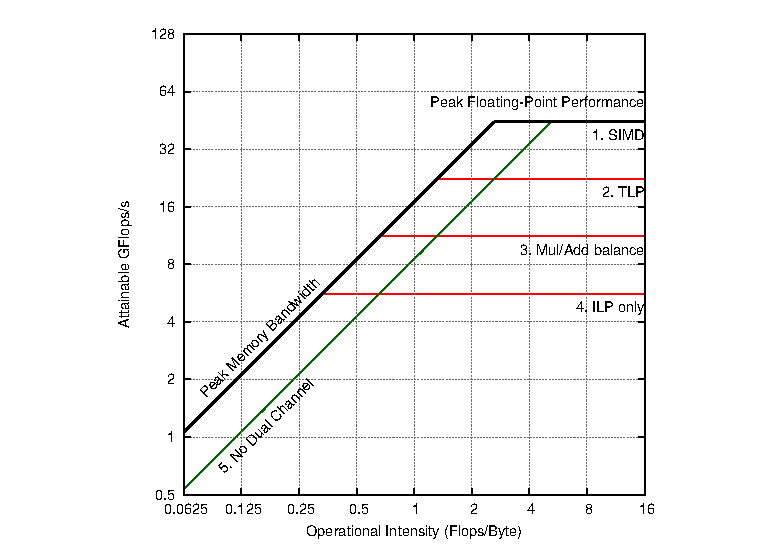
\includegraphics[width=12cm]{images/roofline.eps}
		\label{fig:roofline}
		\end{figure}
\end{frame}

\section{PAPI Case Study: Matrix Multiplication}
\begin{frame}%	begin slide
	\frametitle{Problem}

	Analyse the performance of a \textbf{matrix multiplication} algorithm, \begin{equation}Matrix A * Matrix B = Matrix C\end{equation} wich contains a triple nested loop with the indexes i,j and k (line,column and position).\\

	The implementation used runs two versions of the problem, one multipying matrixA with matrixB, and another multipying matrixA with the transpose of matrixB.
\end{frame}%	end slide

\begin{frame}[fragile]
	\frametitle{Algorithm}

Standard implementation of a matrix multiplication in C.

\begin{verbatim}
for (i = 0; i < size; i++) {
    for (j = 0; j < size; j++) {
        for(k = 0; k < size; k++) {
            acc += matrixA[i][k] * matrixB[k][j];				
            }		
            matrixC[i][j] = acc;	
            acc = 0;
        }
    }
\end{verbatim}
\end{frame}

\begin{frame}
	\frametitle{Counters Used}

	Used counters gathered by PAPI:
	\begin{description}
		\item[PAPI\_TOT\_CYC] Total cycles;
		\item[PAPI\_TOT\_INS] Total instructions
		\item[PAPI\_LD\_INS] Load Instructions
		\item[PAPI\_SR\_INS] Store Instructions
		\item[PAPI\_FML\_INS] Multiply instructions
		\item[PAPI\_FDV\_INS] Division instructions
		\item[PAPI\_VEC\_INS] Vector Instructions
		\item[PAPI\_FP\_OPS] Floating point operations
		\item[PAPI\_L1\_DCA] L1 data cache accesses
		\item[PAPI\_L1\_DCM] L1 data cache misses
		\item[PAPI\_L2\_DCA] L2 data cache accesses
		\item[PAPI\_L2\_DCM] L2 data cache misses
	\end{description}
\end{frame}

\section{Test cases}
\begin{frame}
	\frametitle{Test cases}

	Test cases were selected to fit on the multiple memory levels.\\
	Each Test case was run 4 times for each version of the problem.

	\begin{center}
		\begin{table}[!htp]
	\begin{tabular}{lrlrlrl}
		\hline
		\textbf{Memory} & \textbf{Size} & \textbf{Matrix Size} \\
		\hline
		L1 & 30 KB & 50 \\
		L2 & 255 KB & 146 \\
		L3 & 3 MB & 500 \\
		RAM & 7.68 MB & 800 \\
		\hline
	\end{tabular}
	\caption{Test cases}
	\label{tab:testcases}
\end{table}
	\end{center}
\end{frame}

\section{Results}
\subsection{Memory Accesses}


\begin{frame}
	\frametitle{Memory Accesses}

	The following table shows the number of memory accesses, through PAPI readings.

	\begin{table}[!htp]
		\begin{center}
		{\small
			\begin{tabular}{|l|r|c|}

				\hline
				Test	&	PAPI	&	 Accesses/Inst		\\
				\hline
				L1\_1	&	380844 & 0.49033 \\
				L1\_2	&	258412 & 0.33270 \\
				L2\_1	&	9411279	& 0.42860\\
				L2\_2	&	6318058	& 0.33449\\
				L3\_1   &	7761996 & 0.00885\\
				L3\_2   &   152192 & 0.00020\\
				\hline
			\end{tabular}
		}
		\end{center}
	\end{table}
\end{frame}


\section{Conclusion}
\begin{frame}
	\frametitle{Conclusion}
	\begin{itemize}
		\item Some difficulties measuring memory ceilings;
		\item Lack of analysis of output from PAPI;
	\end{itemize}
\end{frame}

\section{Questions}
\begin{frame}
	\titlepage
	
	
\end{frame}

\end{document}%	end presentation